%
% LaTeX report template 
\documentclass[11pt,onecolumn]{IEEEtran}
%\documentclass[11pt,english]{article}
%\documentclass[journal,11pt,onecolumn]{IEEEtran}
%%%%%%%%%%%%%%%%%%%%%%%%%%%%%% Loading packages that alter the style
\usepackage[]{graphicx}
\usepackage[]{color}
\usepackage{alltt}
\usepackage[T1]{fontenc}
\usepackage[utf8]{inputenc}
\usepackage{mathptmx}
\usepackage{amsmath,amssymb,amsfonts}


 
\usepackage{booktabs}
\setcounter{secnumdepth}{3}
\setcounter{tocdepth}{3}
\setlength{\parskip}{\smallskipamount}
\setlength{\parindent}{12pt}
\usepackage{caption}
\captionsetup[figure]{justification=justified,font=small}
% Set page margins
\usepackage[top=60pt,bottom=65pt,left=68pt,right=68pt]{geometry}
\usepackage{subcaption}
% Package used for placeholder text
\usepackage{lipsum}
\usepackage{booktabs}
\usepackage{multirow}
\usepackage[numbers]{natbib}
% Prevents LaTeX from filling out a page to the bottom
\raggedbottom

% Adding both languages
\usepackage[english]{babel}
\AtBeginDocument{\renewcommand{\bibname}{References}}
% All page numbers positioned at the bottom of the page
\usepackage{fancyhdr}
\fancyhf{} % clear all header and footers
\fancyfoot[C]{\thepage}
\renewcommand{\headrulewidth}{0pt} % remove the header rule
\pagestyle{fancy}
\newcommand{\subparagraph}{}
% Changes the style of chapter headings
\usepackage{titlesec}
\titleformat{\chapter}
   {\normalfont\LARGE\bfseries}{\thechapter.}{1em}{}
% Change distance between chapter header and text
\titlespacing{\chapter}{0pt}{40pt}{2\baselineskip}

% Adds table captions above the table per default
\usepackage{float}
\floatstyle{plaintop}
\restylefloat{table}

% Adds space between caption and table
\usepackage[tableposition=top]{caption}

% add cc license
\usepackage[
type={CC},
modifier={by-nc-sa},
version={4.0},
]{doclicense}

% Adds hyperlinks to references and ToC
\usepackage{hyperref}
% Uncomment the line below this block to set all hyperlink color to black
\hypersetup{
	colorlinks,
	linkcolor={blue},
	citecolor={green!90!black},
	urlcolor={red!70!black}
}
%\hypersetup{hidelinks,linkcolor = black} % Changes the link color to black and hides the hideous red border that usually is created

% Set specific color for hyperref
\usepackage{xcolor}
\usepackage{wrapfig}

% tcolorbox; Notice! add "-shell-escape" to the compile command
\usepackage{tcolorbox}

% If multiple images are to be added, a folder (path) with all the images can be added here 
\graphicspath{ {images/} }

% Separates the first part of the report/thesis in Roman numerals
%\frontmatter
\pagenumbering{arabic}
%
\begin{document}
%
%   \title{A simple template for a lab report}
%
%   \author{P. Archimedes \\ e-mail: archimedes@uni-syracuse.edu}
%          
%   \date{}
%
%   \maketitle
%   
%   \tableofcontents
% 
%  \newpage
    
% This is a comment: in LaTeX everything that in a line comes
% after a "%" symbol is treated as comment

%\section*{\centering{Speaker Extraction based on Deep Learning}}
\title{Multi-objective Reinforcement learning (MORL)}
%\author{Haleh Damirchi, Sanaz Seyedin, and Seyed Mohammad Ahadi}
%\thanks{This paragraph of the first footnote will contain the date on which you submitted your paper for review.}


\maketitle
\section*{\centering\textbf{Toy Tasks}}
The paper used 4 tasks to evaluate the proposed approach, with FTN and DST being simpler that the other two:

\begin{itemize}{
\item Fruit tree navigation task (FTN)
\item Deep sea treasure (DST)
\item Dialog
\item Supermario
}\end{itemize}


Supermario takes a long time to run fully, about a month for 32000 episodes, and the authors had used a cluster of 2080 GPUs so I did not work on it for now. The other task, called the fruit navigation task was simpler and took about 5 hrs to run on google colab. The task is composed of a tree with depth of 5, 6 or 7 (we can choose between them when initializing the tree.). The nodes of the tree are supposed to contain the multi-objective reward for each action taken, which is moving to the right or left branch on in each node. However, in this tree the nodes contain zero reward. The only reward is on the leaves of the tree. Each node on the tree has two branches, and the direction is decided by a DNN. At every run when testing the system, the tree picks a random vector of weights. Then the tree is supposed to guide us to a leaf that would result in the highest $w.r$. This means that the DNN is supposed to learn how to give us the best trajectory when it was given a random weight. Therefore, each trajectory would be dependent on the random weight. 
The picture of the tree is as follows (From \cite{yang2019generalized} appendix):

\begin{figure}[!htb]
    \centering
    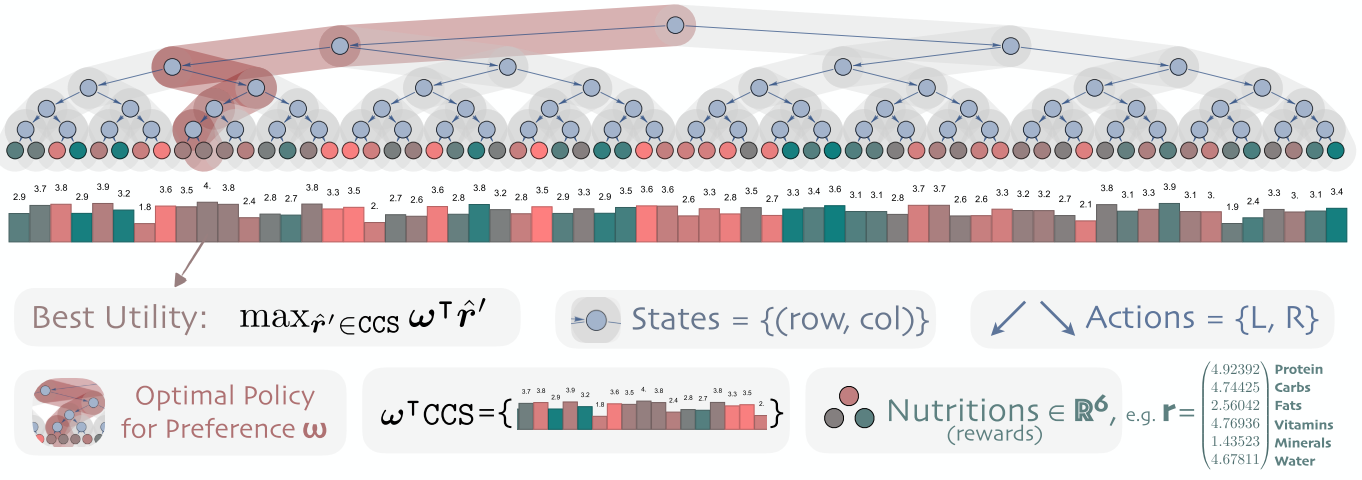
\includegraphics[width=1\linewidth]{tree.png}
    \caption{Fruit Tree Navigation (FTN): An agent travels from the root node to one of the leaf node to pick a fruit according to a post-assigned preference $w$ on the components of nutrition, treated as different objectives. The observation of an agent is its current coordinates (row, col), and its valid actions are moving to the left or the right subtree.}
    \label{fig:blstm}
\end{figure}

The training is illustrated in Fig.~\ref{fig:process}. The process uses double Q learning, in which two models are defined. The reason for this is that, when training the Q network in the deep Q learning method, we use the bellman equation to update the model, and the bellman equation itself uses the model output. It seems like we are chasing to learn a model that is changing itself. So, two models are defined, one target model and one model. The target model is only updated after certain episodes, but the model changes and learns using the loss function. 

\begin{figure}[!htb]
    \centering
    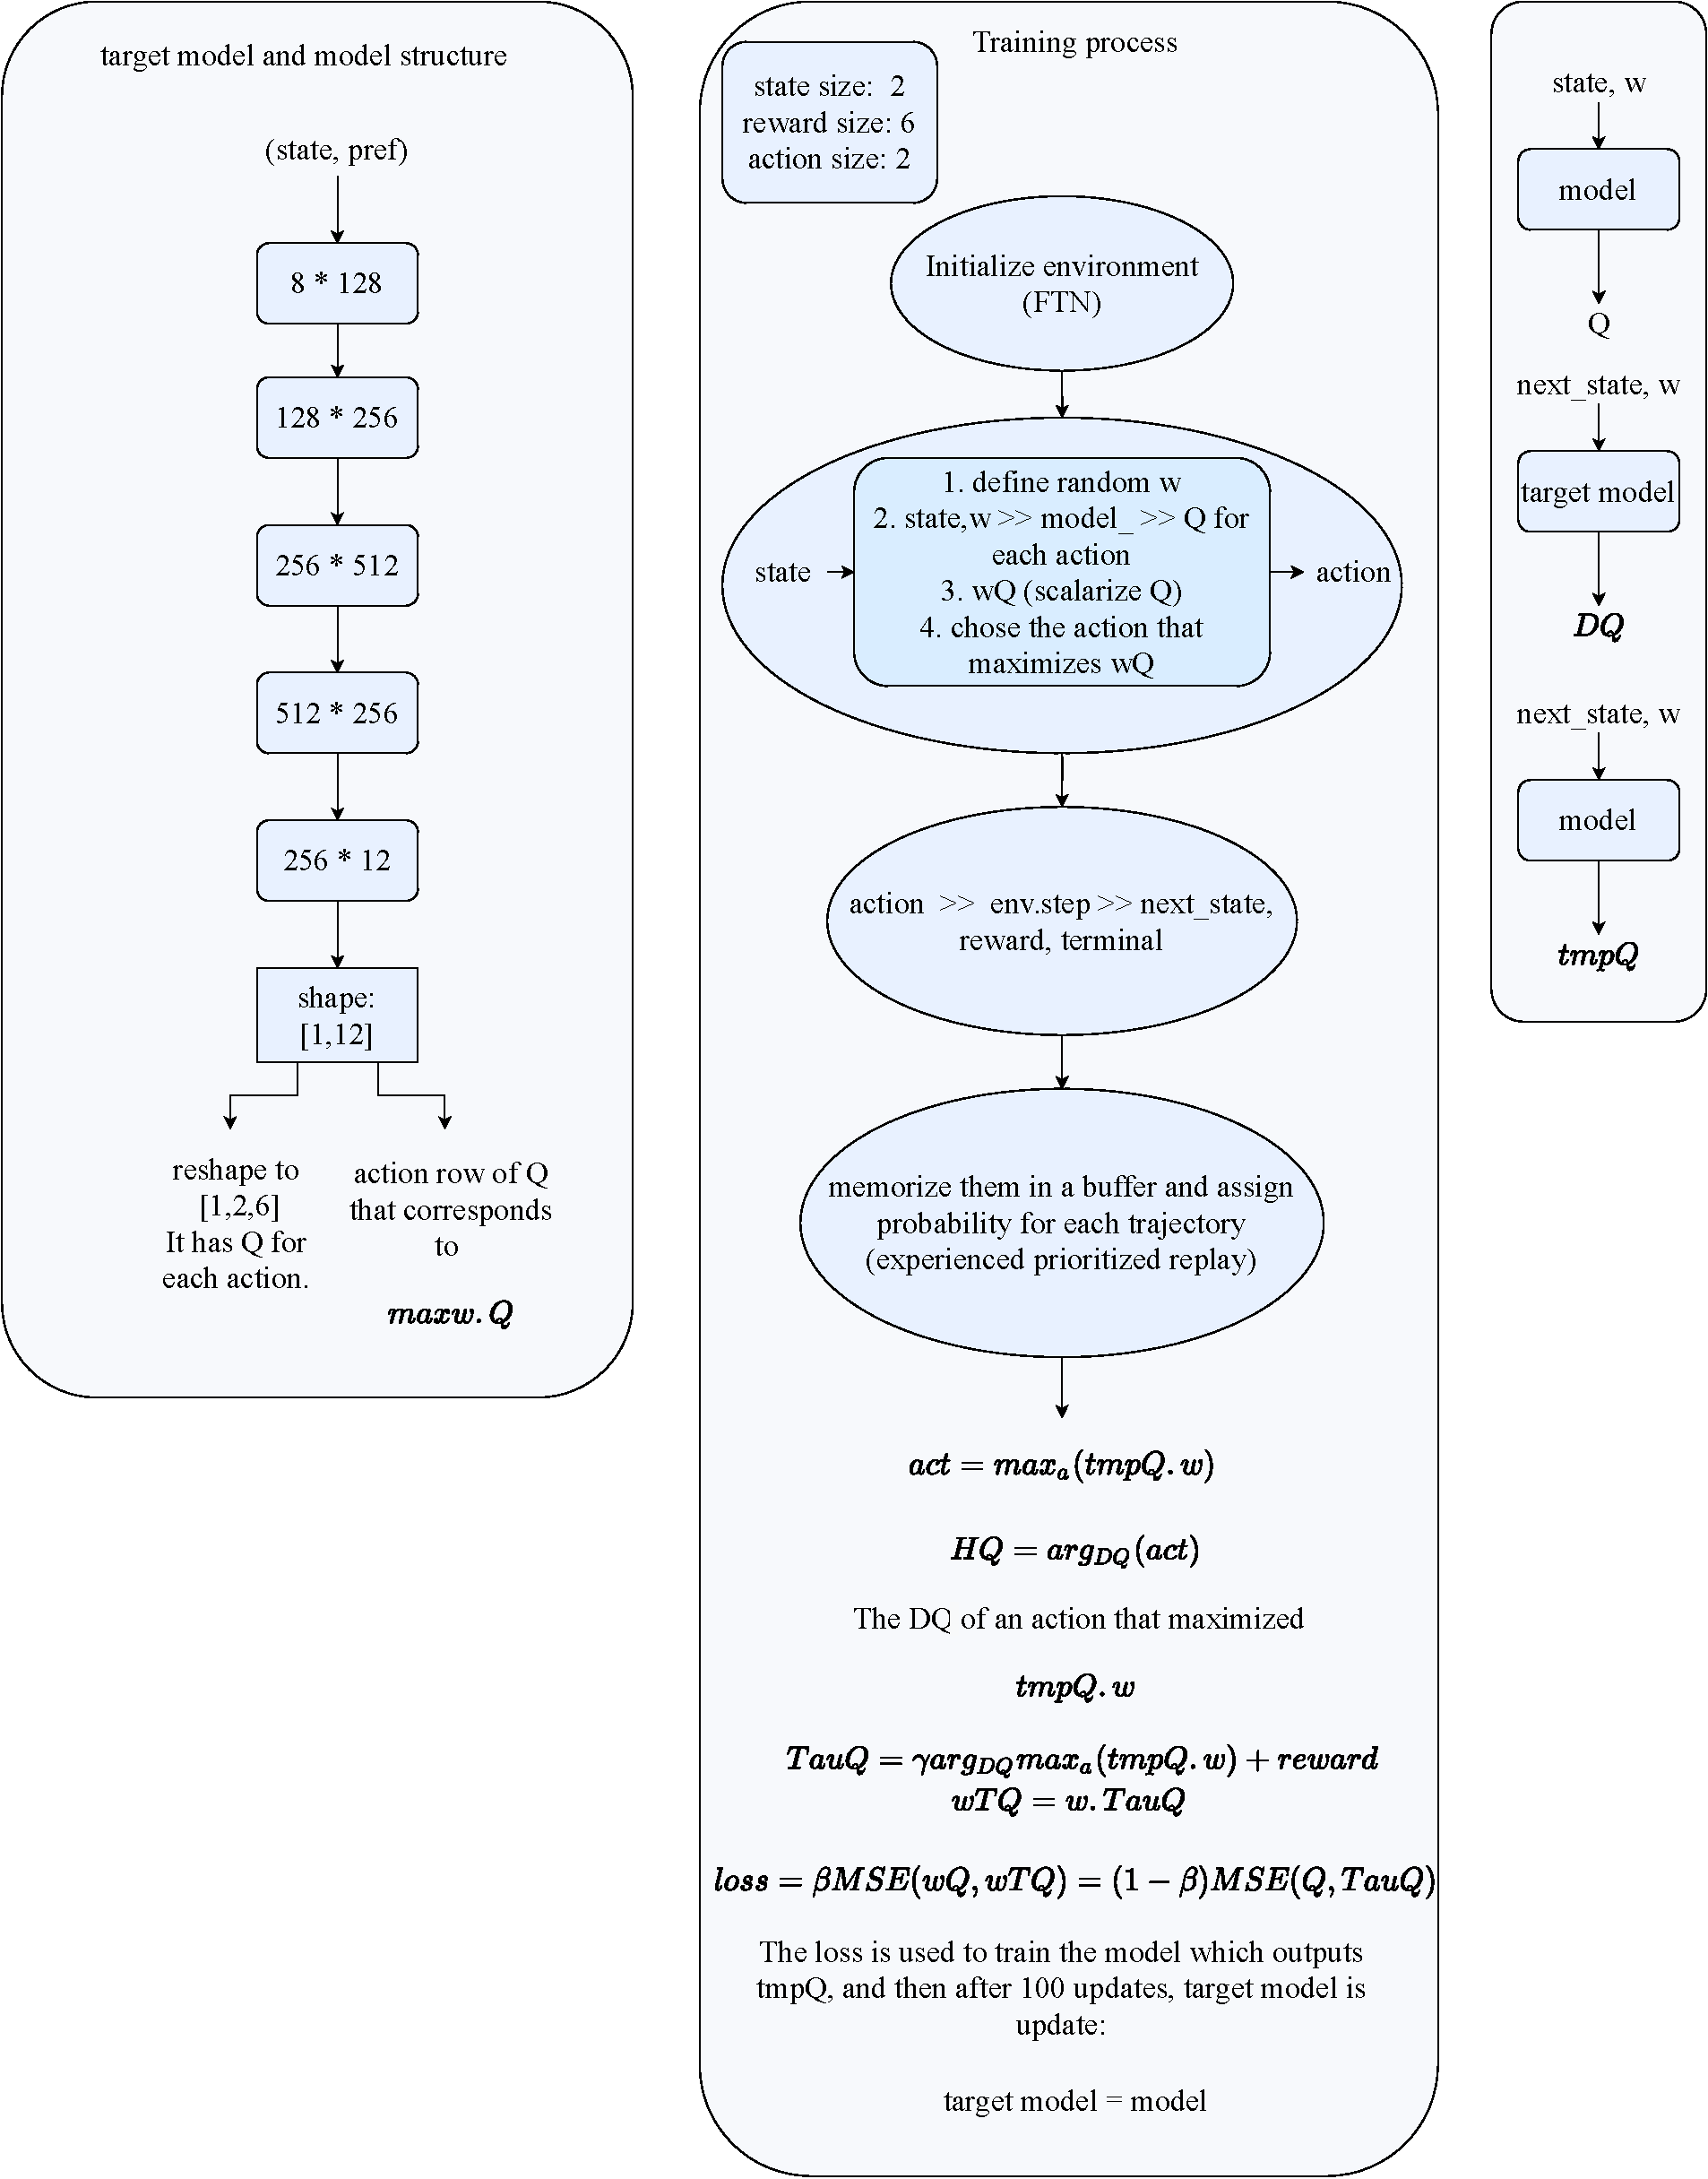
\includegraphics[width=1\linewidth]{process.pdf}
    \caption{The whole process of training MORL.}
    \label{fig:process}
\end{figure}

\section*{\centering\textbf{Implementing the proposed approach}}

As we talked about this in our last meeting, it might be beneficial to let the weights change with a trend like the approach taken in \cite{heydari2019softadapt}. In this paper, there are coefficients for each segment of the loss function. 

\begin{equation}
	\label{jfilt}
		\alpha_{k}^{i} = \dfrac{e^{\beta s_{k}^{i}}}{\sum_{l=1}^{n}e^{\beta s_{k}^{i}}}
\end{equation}

where $s_{k}^{i}$ is the difference between the loss component in the iterations $i$ and $i-1$. when $\beta>0$ the algorithm focuses on improving the worst component of the loss (the part of the loss function that is increasing.) and vice versa. But here, the advantage of using random preferences is that it is random. and it gives the whole process sort of a freedom to chose any weight and get the best result with that weight. However, we can change the mean of the each component of the random weight. In the implementation of the paper, the weights are generated with 0 mean and unit variance normal random function. But if we save the loss and make a list of losses in an inner loop of the process, we can modify the function to define the mean of the random function that is generating the weights. So for example, if the $\beta$ is negative, the random function that is generating the weights for each objective would be likely to assign a bigger number to the objective that had the least loss value. The $s$ here would be the losses itself not the differences between them. Then the mean is saved after training to be used at test time. The proposed approach is explained in Fig.~\ref{fig:proposed} more thoroughly.The red text is the added parts to the main approach.

\begin{figure}[htbp]
    \centering
    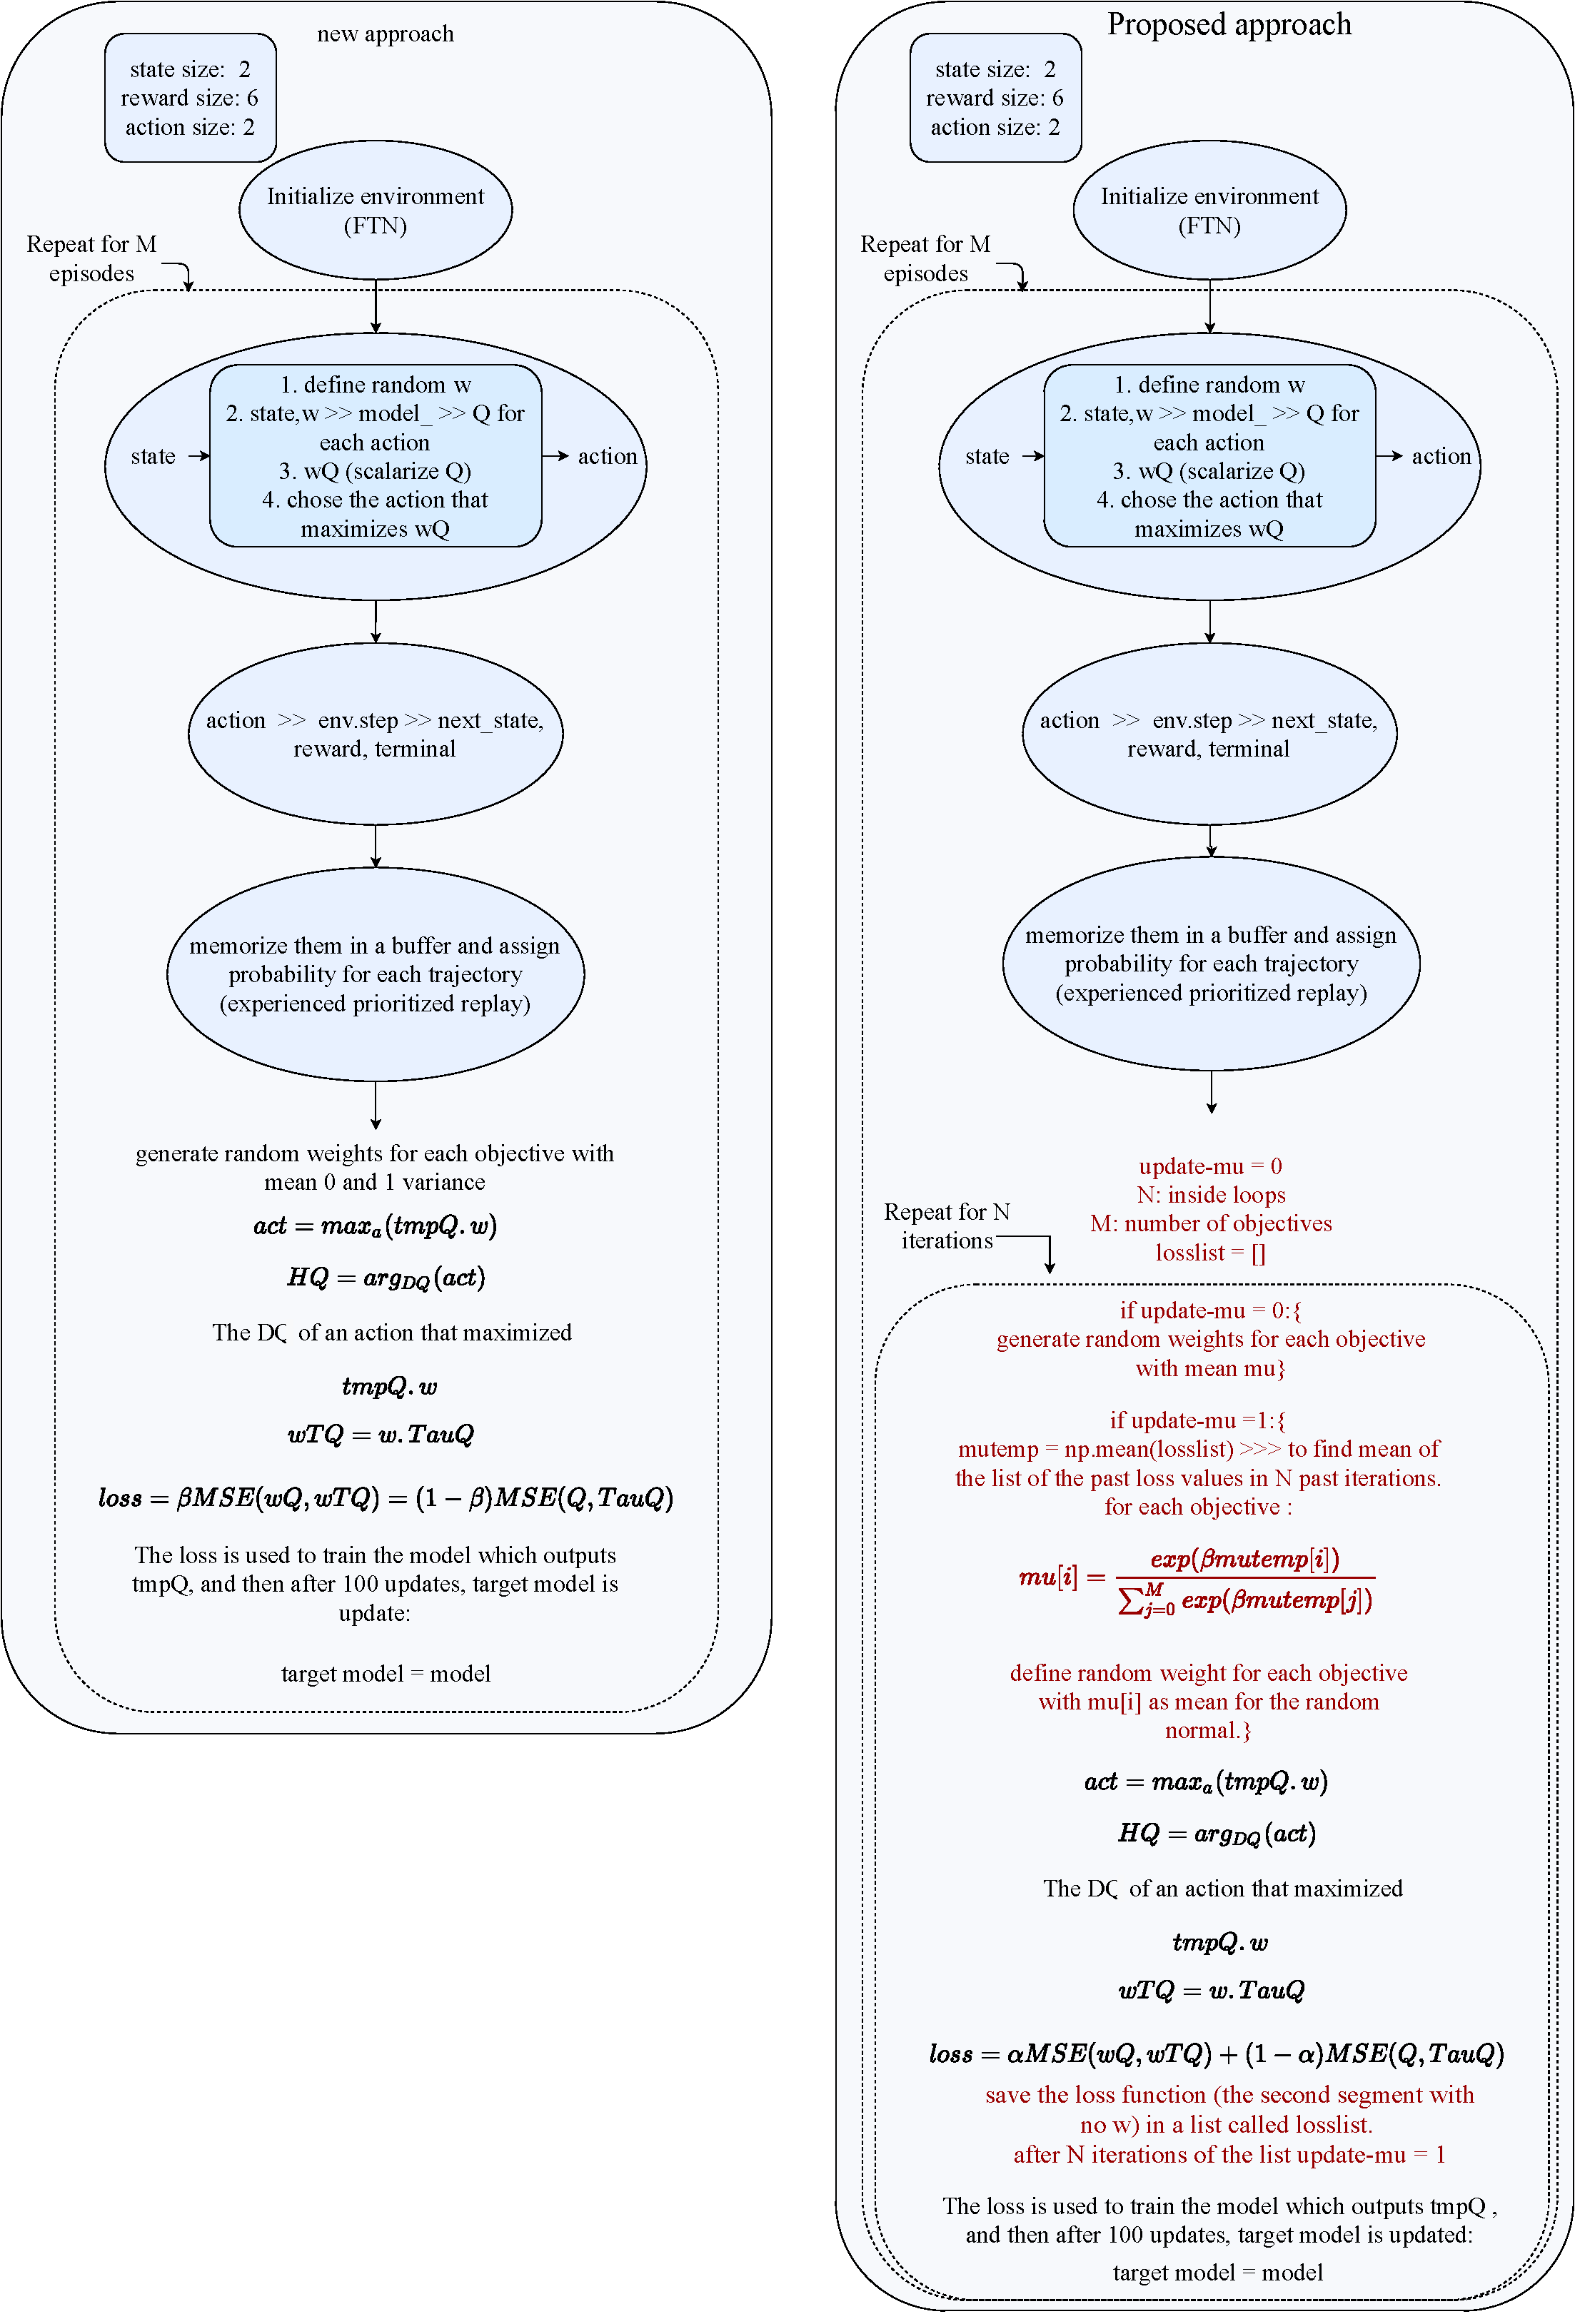
\includegraphics[width=0.9\linewidth]{proposed.pdf}
    \caption{The whole process of training MORL.}
    \label{fig:proposed}
\end{figure}

\section*{\centering\textbf{Experiments}}

The paper uses two evaluation metric. Coverage ration (F1) and Adaptive error. F1 measure how well the trajectories are spread. For instance, when changing the weights, do we get another leaf in the tree or do we end up in a few popular leaves? Adaptive error also finds the error between the $w.r$ of the leaf that was chosen in the test process and the highest $w.r$ from the tree. So it tries to find out if we got to the leaf that would result in the largest value after multiplying the weight in the multi-objective reward. 

The loss functions for both approaches are depicted in figure Fig.~\ref{fig:full_loss} and Fig.~\ref{fig:partial_loss}. The loss is noticeably lower in our proposed approach in the last episodes. However, there is a dip in the loss value around episode number 3000. I will run this again for 5 times to average the results and see if it happens again. It might be due to saving the wrong log files in between since google colaboratory crashed once in a while and the training needed to be continued. The loss value is also highly unstable at the beginning when looking at the proposed approach but it gets better at the end compared to MORL. However, there is an important point here that we trained the network for $N$ more times (the inner loop) in each episode. The run time for the MORL was about 4-5 hours and the runtime for the proposed approach was 9-10 hours with $N=9$. So the runtime did not increase that much. But it might also be that the adaptive mean assignment for random function generating the weight for each objective does not have much effect in the improvement of the evaluation results. maybe having that inner loop causes the network to be trained more with the random weights (In MORL the network is only trained once with the random weights but here we trained it for 9 times with the same random weights.) That would also explain why the ups and downs are much less in the new approach.In another version of the model, the loss is switched. Meaning that $\alpha$ and $1-\alpha$ have switched places in the loss function. By doing that the network first tries to optimize the second section of the loss function and then gradually moves toward optimizing the first section. But I suppose comparing the loss value for this approach with the two other ones does not show anything since the formula for loss function is different here.
\begin{figure}[htbp]
    \centering
    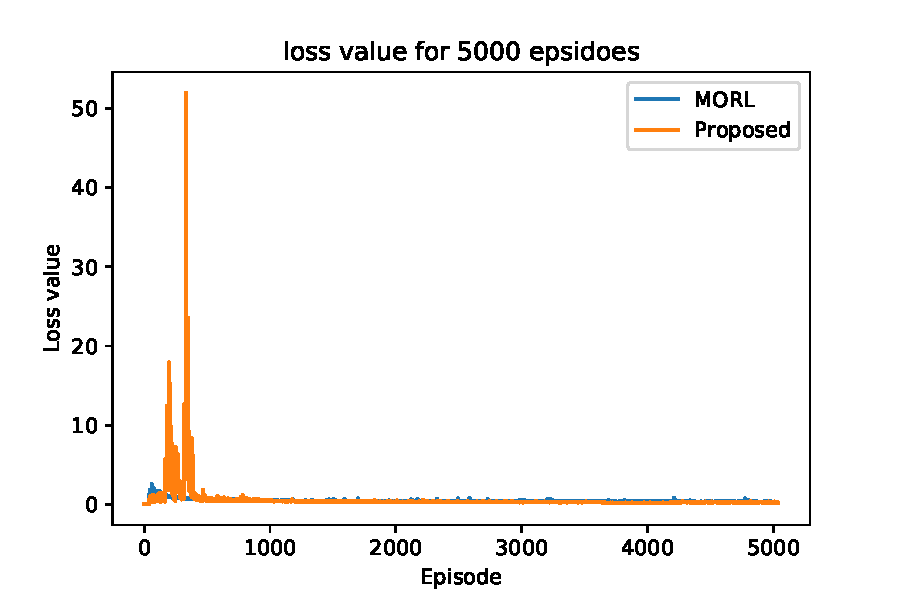
\includegraphics[width=0.7\linewidth]{full_loss.pdf}
    \caption{Loss value of the MORL and proposed approach in 5000 episodes of training.}
    \label{fig:full_loss}
\end{figure}

\begin{figure}[htbp]
    \centering
    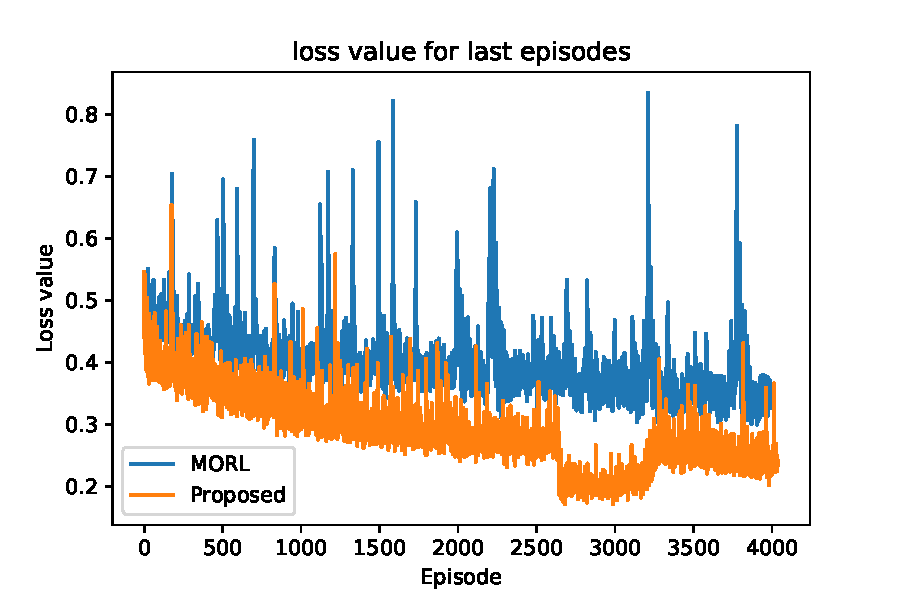
\includegraphics[width=0.7\linewidth]{partial_loss.pdf}
    \caption{Loss value of the MORL and proposed approach in the last 1000 episodes of training.}
    \label{fig:partial_loss}
\end{figure}
Also, the F1 and AE results for the approaches discussed above as well as the approach in the paper is depicted in Table~\ref{tab:eval}. The downward arrow mean that lower values are better and vice versa. The new approach improved the F1 and AE value. The switched loss approach could not improve the F1 but could somewhat improve the MORL approach. The code is forked from the main github, and is under MORL-colab: \href{https://github.com/thisishale/MORL}{Colab code directory}



\begin{table}[htbp]
\centering
\caption{}
\begin{tabular}[t]{lcc}
\toprule
& Adaptive Error (100$\times$error) $\downarrow$  & F1 $\uparrow$ \\
\midrule
 MORL & 1.2021 & 0.98567  \\ 
 Proposed approach & 0.8104 & 0.99685 \\ 
 Switched loss & 1.0342 & 0.96430 \\ 
\bottomrule
\end{tabular}
\label{tab:eval}
\end{table}%
\medskip
\clearpage
%\section*{References}
\bibliography{references}
\bibliographystyle{IEEEtran}
\end{document}



